\chapter{Preliminary Case Study}

The Tezos blockchain has proven itself to be a flexible and adaptable platform, capable of accommodating a wide range of applications and use cases. This makes it a suitable choice for an experiment that aims to test and demonstrate the implementation of a consensus protocol. In this chapter, we will elaborate on why Tezos is an ideal fit for this experiment and explore the inner workings of the platform that make it so.

The experiment at hand involves the implementation of a Proof of Work consensus protocol, similar to the one used by the Bitcoin blockchain.
As an exercise, this protocol was implemented on the Tezos blockchain and its workings will be discussed in detail. This will include a discussion of the requirements for a protocol, its integration with the Tezos node, the implementation of the protocol itself and the tools used to interact with it.

We will also delve into the implementation of a client and a baker, which are integral components of the protocol. The client is used to access information within the network, while the baker is responsible for the creation and mining of blocks. This includes the process of mining the block by finding the nonce that makes the block's hash lower than the target, which is a key point in the execution of a Nakamoto like consensus.

In conclusion, this experiment will serve as a demonstration of the flexibility and adaptability of the Tezos blockchain and its ability to accommodate different consensus protocols. The implementation of the Proof of Work consensus protocol will serve as a proof of concept and highlights the potential of the platform to support a wider range of consensus protocols, even those different from the orginal protocol implemented.

\section{Tezos Blockchain as a tool for the Experiment}
The choice of Tezos as the blockchain network for this experiment is a deliberate one, as it aligns well with the goals of the solution presented in the previous section.

To understand why Tezos was chosen, it is important to first explain what Tezos is.
Tezos is a blockchain network that was launched in 2018, and it's history began with the idea of creating a generic and self-amending crypto-ledger, which could be improved and upgraded over time without causing any disruption to its community. This makes Tezos stand out from other blockchain networks, which often struggle with the challenges of upgrading their underlying technology. 
The idea behind it is to provide a blockchain network that is not only secure, but also flexible and upgradable. The network is designed to be self-amending, meaning that changes to its protocol can be made without the need for a hard fork. 
Tezos originally operates on a Delegated Proof of Stake consensus, but the specifics of this consensus are irrelevant since we are taking it out and swapping with different consensus protocols.

A hard fork is a permanent divergence in the blockchain of a cryptocurrency, leading to the creation of two separate chains. It occurs when a node's existing code is altered, resulting in a change to the rules that govern the network. 
This can happen for a variety of reasons, including a desire to add new features to the network, fix security vulnerabilities, or resolve a disagreement within the community about the direction of the project. The disagreement of the size of a block in Bitcoin was the cause of a creation of Bitcoin Cash's network (mentioned in example \ref{bitcoincashexample}), where the Bitcoin blockchain was splitted in two (and later in more chains).

When compared to other blockchain networks, Tezos stands out as a really good fit for this experiment. It is commercially, well-tested and industry-grade blockchain network, and its upgradability makes it suitable for the replacement of the consensus algorithm. Additionally, the protocol in the codebase is independent and the whole project is designed for the replacement of such. 
The idea of the protocol/consensus layer in Tezos is that it's stateless, meaning that it is independent from other parts of the node like the Peer-to-Peer layer, the client, the validation layer, and the storage of the blockchain state on disk.
This makes it easy to focus on writing the actual protocol and eliminates the need to worry about other components.


In conclusion, using Tezos for this experiment was a strategic decision as it offers the necessary features and characteristics to carry out the experiment successfully. Its history, design, and upgradability make it an ideal candidate for this experiment, and the stateless nature of the protocol part of the codebase allows the focus to be on the consensus, rather than other components of the node.
The results of this experiment will provide valuable insights into the potential of Tezos and its adaptability, making it an exciting step in the development of a blockchain network that can easily swap consensus algorithms.



\section{How Tezos is structured and How it allows self-amending}

Tezos has a unique structure, which separates the protocol, or how the Tezos project calls it, ``Economic Protocol'' from the rest of the node, known as the shell. The diagram \ref{fig:octupus} illustrates the Tezos architecture, and it's explained in greater detail here \cite{nomadiclabsdocs}.
The protocol is responsible for interpreting transactions and administrative operations, as well as detecting erroneous blocks, everything else is handled by the shell.

The shell includes the part of the validation code, the peer-to-peer layer, the disk storage of blocks, and the versioned state of the ledger.
The distributed database abstracts the fetching and replication of new chain data to the validator.

The economic protocol on the chain is subject to an amendment procedure, which allows for the on-chain operations to switch from one protocol to another.

Finally, the RPC (Remote Procedure Call) layer is an important part of the Tezos node, allowing clients, third-party applications, etc. to interact with the node and introspect its state using the JSON format and HTTP protocol.

In other words, the outside world of the node communicates with the shell, via RPC layer calls, and the shell communicates with the protocol. Like said previously, the protocol is stateless, and is only used to preform the logic part of the consensus, that is, to verify transactions, blocks and to describe what the shell should do when receiving newer information.

The communication between the shell and the protocol in Tezos is based on an interface called ``Updater.PROTOCOL''.
The protocol component is restricted to a specific environment that restricts the access to a defined set of OCaml modules. This is to improve the security of the protocol.
The protocol must implement the ``Updater.PROTOCOL'' interface (defined in the environment, and later explained in more detail) in order to interact with the shell. The interface requires the protocol to define protocol-specific types for operations/transactions and block header, along with encoders/decoders for the types.

The protocol must also provide functions for processing blocks and updating the context, which represents the protocol state. The context is stored as a disk-based immutable key-value store. The block header and operations also have a shell header (protocol-independent) and a protocol-specific header.
For example, a Block can have two levels, one corresponding to the overall/shell level, and other is the level of the block since the current protocol is started.

Blocks in Tezos have a generic part, understood by any protocol, and a protocol-specific part.

A Tezos node can contain multiple economic protocols, but only one of them is activated at any given time, and the it always starts with the ``genesis'' protocol.

Some protocols are linked to the node at the time of compilation, that is, the node already has information about it when starting, and some protocols can also be registered dynamically at runtime via an RPC, allowing for protocol updates without the need of manual intervention to do so.

Protocol activation in Tezos is a two-step process.

Firstly, a command injects an ``activation block'' to the blockchain. This block contains the hash of the protocol to be used, and only one operation to activate it. The activation block is the only block using the genesis protocol, as this protocol doesn't contain any other functionality besides the activation of a different protocol.

Secondly, the next block in the blockchain will be the first block using the activated protocol. 


\begin{figure}[H]
    \centering
    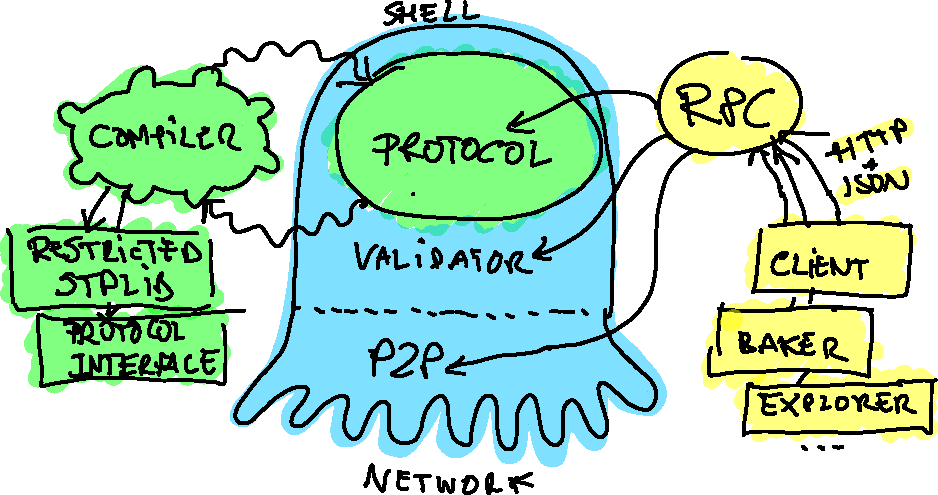
\includegraphics[width=\textwidth,keepaspectratio]{imagens/octupus.pdf}
    \caption{Architecture of Tezos (Source: Tezos Documentation)}
    \label{fig:octupus}

\end{figure}

In conclusion, the structure of Tezos is unique in that it separates the protocol, also known as the ``Economic Protocol'', from the rest of the node, called the shell. The protocol is responsible for interpreting transactions and administrative operations, while the shell includes the validator, peer-to-peer layer, disk storage of blocks, and versioned state of the ledger. The economic protocol on the chain is subject to amendment procedures, allowing for on-chain operations to switch from one protocol to another. The RPC layer allows clients, third-party applications, and daemons to interact with the node and its state. The communication between the shell and the protocol is based on the Updater.PROTOCOL interface, and the protocol is restricted to a specific environment to improve security. A Tezos node can contain multiple economic protocols, but only one of them is activated at any given time through a two-step activation process.


\section{Implementation of a Protocol}

Implementing a Proof of Work consensus algorithm as a protocol for Tezos was motivated by several reasons. Firstly, it was an opportunity for hands-on learning about how protocols are implemented and structured. This understanding is crucial for later work, such as testing and adding an adaptive layer to the DSL mentioned in previous sections. It was necessary to understand how these protocols work before attempting to create tools related to them.
It also allowed for a deeper understanding of how Tezos works as a whole.

The implementation of Proof of Work was also significant because it provides a contrast to Tezos' original Proof of Stake protocol. This demonstrated that Tezos can be used to implement other types of consensus algorithms, including those that are different from the original. The implementation of Proof of Work also has the concept of mining, which is not present in the Proof of Stake protocol.


Additionally, implementing a protocol in Tezos is a big accomplishment. The fact that only a few people do so makes this achievement even more significant, especially considering that it's a different type of consensus. This demonstrates a deep understanding of consensus algorithms and the ability to put that knowledge into practice.



In conclusion, the implementation of Proof of Work as a protocol for Tezos was a valuable learning experience that allowed for a deeper understanding of how protocols are structured and executed in Tezos. It also reinforced the concept of consensus algorithms and demonstrated the ability to put that knowledge into practice by implementing a unique protocol in Tezos.


\subsection*{Requirements of a Protocol In Tezos}
In order to implement the experiment of a Proof of Work consensus algorithm for Tezos, a "lib\_protocol" module in the protocol folder had to be created, where this is the main entry to the protocol and is executed by the node as the new amendment/consensus protocol. This is the only part that has to be implemented in OCaml and has to be compiled to work with the node.

To do so, a ``TEZOS\_PROTOCOL'' file must be included in this module, that is used to specify the version of the environment that the protocol is to be compiled against, which in this case the version 6 was the one used, the hash of the protocol folder and the set of modules implemented in the folder. 

There's the possibility to implement a newer environment for the protocol to accommodate the protocol, yet, for this experiment, this wasn't necessary. 

Like said previously, the environment is an interface that provides a set of OCaml modules that the protocol can use, and the interface used to interact with the Tezos Shell.

The most important functions and types in that had to be implemented for environment ``v6'' were:

\begin{itemize}
    \item \emph{block\_header\_data}: This is the protocol-specific part of the header.
    \item \emph{block\_header}: This is the combination of the protocol header and the shell header.
    \item \emph{operation\_data}: This is the protocol-specific part of an operation/transaction.
    \item \emph{operation}: This is the combination of the protocol operation part and the shell operation part.
    \item \emph{validation\_state}: This is the state of the validation of a block or operation, passed between functions.
    \item \emph{init}: This function is executed to prepare the chain to start executing the new protocol.
    \item \emph{begin\_application}: This function is used when validating a block received from the network.
    \item \emph{begin\_partial\_application}: This function is used when the shell receives a block more than one level ahead of the current head. 
    \item \emph{begin\_construction}: This function is used by the shell when instructed to build a block and for validating operations as they are gossiped on the network.
    \item \emph{apply\_operation}: This function is called after \emph{begin\_application} or \emph{begin\_construction} and before \emph{finalize\_block} for each operation in the block or in the mempool, respectively. It validates the operation and updates the intermediary state accordingly.
    \item \emph{finalize\_block}: This function represents the last step in a block validation sequence.
\end{itemize}

In summary, the ``TEZOS\_PROTOCOL'' file is used to specify the protocol environment to be used by the Tezos node, and the environment provides a set of functions and types that the protocol must implement to be able to operate within the Tezos network.

\subsection*{Implementation of the module ``lib\_protocol''}

The implementation of a new protocol in the Tezos codebase is a significant challenge.
In this particular case, the goal was not only to implement the new protocol, but to also learn how existing protocols are structured and implemented within the Tezos codebase. The approach was to study and follow closely the implementation of existing protocols, rather than taking an easier approach that may also have resulted in a working protocol but would not have offered the same level of learning.

The protocol that was implemented includes a few functionalities, such as transactions between two entities, where ``Tez'', the currency used in Tezos, is transferred from one account to another.

Another aspect of the protocol is the concept of mining and verifying the proof of work, like mentioned in a previous section about Proof of Work.
This is done by hashing the header whole header, both the shell part and the protocol part, this last one containing the nonce, and verifying that the hash value is lower than the target where this is one of the main mechanism behind proof of work.

The environment that the protocol is compiled against requires a definition of the protocol header, which contains three elements: ``target'', ``nonce'', and ``miner''.

The \textbf{target} is used for comparison with the target value that the node calculated it should be (the specifics of how this is done is explained in a later point).
The \textbf{nonce} is used to achieve a header hash with a value lower than the target, which is a key part of the Proof of Work mechanism.
Finally, the \textbf{miner} field stores the address of the miner who found the nonce/hash, which is used to reward the miner. These elements combined make up the protocol-specific part of the header.


\subsection*{Implementation of Information Representation and Storage Logic}

The implementation of the protocol in Tezos involves defining and representing the various types of information that are necessary for the protocol to function. This includes things like accounts, constants, headers, time, target, currency (Tez), and operations.

The information stored in the protocol is abstracted, meaning that the protocol itself is stateless. The context in which the protocol is applied maps to the actual storage of the blockchain, but this is hidden from the protocol. The protocol only sees the storage as a generic key-value store and the functions that access this are defined in the "raw\_context.ml" file (in reality, they are accessed as a Tree, not just as a generic key-value). These functions allow the protocol to read, write, and update the storage, but the actual details of how this is done are not relevant to this document.

Also, as mentioned previously, the shell part of Tezos doesn't necessarily ``understand'' the protocol, as the protocol is somewhat independent from it. So the way that Tezos handles this fact is by representing the protcol parts of data (either from Blocks, Storage or Operations) as bytes, then these bytes are decoded by the protocol.

The encoding and decoding process of this information is done using the ``data-encoding'' library in Tezos. This library is also used to encode and decode OCaml types to and/from bytes or JSON, so it can also be sent to other nodes in the network.

The Tezos Protocol is implemented through a series of files that represent various components and functionalities. In this section, we will take a closer look at the information stored and the logic behind each component in the protocol.

The protocol contains representations/definitions and operations of the following types/\\information, which are stored in files that end with ``repr.ml''. 
The Tezos documentation calls this the ``representation layer'' of the protocol. Unless the representations are only used within the protocol code, they also implement the encoding and decoding logic so this information can be sent/received, either from\/to the network or the shell part of the node.

\begin{itemize}

    \item Accounts/Manager: This represents the concept of an account in the protocol. An account is just a Publick Key Hash, which is used to fetch information from the storage. 

    \item Constants/Parameters: This file contains information that is constant throughout the execution of the protocol. Some constants can be defined when activating the protocol. The constants include:

        \begin{itemize}
            \item \emph{block\_time}: Defines the time between blocks.
            \item \emph{initial\_target}: Defines the first target value.
            \item \emph{difficulty\_adjust\_epoch\_size}: Defines the number of blocks to wait to then readjust the target.
            \item \emph{halving\_epoch\_size}: Defines the number of blocks to wait to then halve the mining reward.
            \item \emph{reward\_multiplier}: The initial reward, which then gets halved.
            \item \emph{Header}: Defines the Protocol header, as mentioned before.
            \item \emph{block\_time}: Defines the time between blocks.
        \end{itemize}
        These parameters are crucial for achieving the project's objective, allowing for more precise tuning of the protocol.

    \item Time: Type definiton of ``time''' in the protocol.

    \item Target: Defines how the target, used in Proof of Work is represented, in this case, it's a 256-bit number.

    \item Tez: Defines the type and operations for the currency.

    \item Operations: Representations and functionalities of the available operations. These include Transactions (between two entities) and Reveal (maps a Public Key to a Public Key Hash, like the ones used in the Accounts).

\end{itemize}

Some of these representations where designed by following the existing protocols implemented in the Tezos codebase. These representations ensure that the creation, conversion, encoding and decoding and other functionalities are done correctly by the protocol.

The logic behind storing information in the Tezos Protocol is an integral part of its functionality. The protocol uses an abstraction over the blockchain as its storage mechanism. 

This is really important to the implementation of the protocol. While implementing a protocol, the developer doesn't have to understand how the blockchain will be stored, what optimizations for inserting and retrieving information are done, etc.

The files that are responsible for storing information have names ending with ``-storage.ml'', and they store the following key pieces of information:

\begin{itemize}
    \item Accounts: It stores information about each account in the protocol. It maps the account's key to the account's balance and other important information and how defines how this information should be stored, retrieved and other checks.

    \item Target: It stores the current target, which is used for comparing the value of the header hash in the proof of work process.

    \item Epoch Time: It stores the timestamp of the latest difficulty adjust epoch, which is used to determine when it's time to adjust the target value. This is an important part of maintaining the security and integrity of the network, as it allows the network to dynamically adjust the difficulty of mining to ensure a stable rate of block production.
\end{itemize}

By storing these types of information in the blockchain, the Tezos Protocol provides a secure and transparent method of tracking the state of the network, which is crucial for the proper functioning of its operations. The protocol also provides a well-defined structure for the information it stores, which ensures consistency and maintainability of the code.

From the Protocol side of view, it sees the Blockchain as a Map/Tree, where it can fetch and append information to it using the typical concept of a Map (in programming).

\subsection*{Implementation of the main entry points to the protocol}

The implementation of the main functions of the protocol plays a crucial role in ensuring the correct execution of the protocol.

These functions are designed to take the necessary steps to apply the information and verify the validity of the information being applied. The functions presented in the previous section, such as \emph{begin\_application}, \emph{begin\_partial\_application}, etc. are all a part of the main functions of the protocol.

These functions perform various checks and updates to the context, which is an immutable representation of the state of the protocol.
The context contains information such as the accounts, the target, and the epoch time, among others. The functions return some form of validation state and updated context, if applicable.

Once again, the protocol is independent from the rest, so these functions are implemented with this concept. 
That is, they are called by the shell part of the node, by passing information such as the current ``context'' and some information about the previous block (to the one being built or validated).



\begin{itemize}

    \item \emph{begin\_application} and \emph{begin\_partial\_application}:
        \begin{itemize}
            \item These functions prepare the current raw context, which contains information such as the context and more. The concept of raw context will be explained later.
            \item Checks are performed, such as verifying if the current target is the correct one and if the header has a valid hash, that is, if the hash of the whole blockheader has a value lower than the target.
            \item They update information such as the target for the next epoch, if an epoch has elapsed.
            \item These functions are called when receiving a block from the network. The partial variant is used when the block received doesn't have the successor level to the current block.
        \end{itemize}

    \item \emph{begin\_construction}:
        \begin{itemize}
            \item Does the same preparation to the context as \emph{begin\_application} and \emph{begin\_partial\_application}.
            \item Performs the same checks, but also rewards the miner if the block is valid.
            \item This function is called when the node is building a node. For example, if the node is a mining node.
        \end{itemize}

    \item \emph{apply\_operation}:
        \begin{itemize}
            \item Verifies if the operation contains a valid signature.
            \item Verifies if the operation has a positive result, for example, if the account has enough funds to transfer to another account.
            \item If the operation is positive, it executes the operation on the current context.
            \item This function is used after both \emph{begin\_application} and \emph{begin\_construction}.
        \end{itemize}

    \item \emph{finalize\_block}:
        \begin{itemize}
            \item Commits the change to the shell.
            \item Returns a receipt or result log that exposes what happened with the application of either a block or operation.
        \end{itemize}
    \item \emph{init:}
        \begin{itemize}
            \item Initializes everything needed to start the protocol, such as the constants and storage.
            \item Also creates the first blocked of the protocol to be appended to the chain.
        \end{itemize}
    \end{itemize}


In high-level view, the way that these functions are executed is the following: 

We assume that every function is independent and purely functional. Each call of any of these functions receive and return (back to the shell) an updated-copy of a value called ``context'', in other words, it updates the state of the blockchain, unless something goes wrong, which then the updated context gets ignored.
The shell handles the flow of execution.
It starts with \emph{begin\_application}, \emph{begin\_partial\_application} or \emph{begin\_construction}, depending of the conditions mentioned above. They handle the initial validation of the block header.

Then, for every operation included in the block, \emph{apply\_operation} is executed, copy-updating the context and passing it to subsequent calls of this function, until the last operation. Here, operations update the state and are validates.

After the last operation is validated, the context is finally passed to \emph{finalize\_block}, where the last updates to the context are performed and the last validations are done. After this function is called (and depending on the result of this process), the block is commited back to the shell, which is then added to the underlying blockchain.



\subsection*{Implementation of Alpha and Raw Contexts}

The implementation of the protocol relies heavily on two core abstractions: \textbf{Alpha\_context} and \textbf{Raw\_context}. These two modules play crucial roles in ensuring the separation of concerns and allowing the protocol to be implemented over a generic key-value store.

Alpha\_context, defined in the ``alpha\_context.ml'' module, serves as the consensus view of the context. This module enforces the separation between mapping the abstract state of the ledger to the concrete structure of the key-value store, and implementing the protocol over the state. The Alpha\_context defines a type ``t'' that represents the abstracted state of the ledger and can only be manipulated through the use of selected manipulations, which preserve the well-typed aspect and internal consistency invariants of the state.

The abstracted state is read from the disk during the validation of a block and is updated by high-level operations that preserve consistency. Finally, the low-level state is extracted to be committed to disk. This abstraction provides a well-separated structure in the code, with the code below Alpha\_context handling the ledger’s state storage, and the code on top of it implementing the protocol algorithm using plain OCaml values.

Raw\_context, defined in the ``raw\_context.ml'' module, is the information view used by Alpha\_context. It serves as the raw, storage, or non-abstract view of what is actually done in the background by the consensus/protocol. Raw\_context provides the abstraction used by Alpha\_context to access the raw part of the protocol, that is, the information that is actually stored and the representation layer.

In conclusion, the implementation of the protocol relies heavily on Alpha\_context and Raw\_context to enforce separation of concerns and to abstract away the underlying implementation details, allowing the protocol to be implemented over a generic key-value store in a readable and well-separated manner.

\subsection*{Features that weren't implemented}
In this feasibility study, we have focused on the implementation of consensus protocol in the Tezos node. However, there are a few features that have not been included in this study but could be considered as future work.

One of the missing features is the support for smart contracts. This was not the main focus of the experiment, but smart contracts can be added on top of the protocol to provide more functionality. Currently, the protocol only supports peer-to-peer value transactions, but with the addition of smart contracts, more complex operations can be performed.

Another missing feature is the lack of upgradability in the protocol. This was intentional as this experiment was focused on a standalone Proof of Work consensus algorithm, and there is no previous protocol nor will there ever be a next protocol that is an amendment to this one. Upgradability could be added to the protocol in the future to provide more flexible and dynamic updates, but once again, for this kind of experiment, doing so would be useless.

It should be noted that the absence of these features was not due to technical limitations, but rather a deliberate decision to focus on the implementation of a protocol in the Tezos.

\section{Tools developed to interact with the protocol}

In this study, tools related to the protocol were also implemented to enable interaction with the network. These tools could be developed independently from the Tezos project, since it's possible to communicate with the tezos node through JSON RPC. However, implementing these tools using OCaml and Tezos modules has the added benefit of being automatically integrated with the Tezos node client (and much more). Upon activation of the protocol, the client would automatically adapt to accommodate it, enabling commands that are specific to the protocol, such as ``Transfer'' and ``Reveal'', which is the case of the protocol covered here.

One of the tools implemented was the client, which can be found in the ``lib\_client'' folder. The client is mostly used to access information on the network, such as an account's balance or the current target. It serves as a better user interface for accessing the information through JSON RPC services. The client also has the capability of injecting blocks and operations into the network, so it can perform the two operations included in the protocol.

Another tool that was implemented is the baker, which can be found in the "lib\_baker" folder. The baker uses functionalities implemented in both the client module and the "Shell Services" module, this last one being already part of the Tezos codebase.
The baker performs the task of baking (how block creation is called in Tezos), or mining, a block by taking multiple operations, pre-applying the block in the protocol (to check if the block header is valid), and then performing the work to find the nonce that makes the block's hash lower than the target, similar to what a miner would do in a Proof of Work blockchain. Once the block is mined, it is pushed to the chain (and spread to the network).

\section{Conclusion}

MUDAR:
In conclusion, this experiment proved to be a valuable exercise as it allowed us to gain a deeper understanding of how consensus protocols work and how they can be implemented within a blockchain network. The implementation of the protocol allowed us to test its capabilities, limitations and to identify areas for improvement. Furthermore, it demonstrated the versatility and flexibility of the Tezos network in accommodating custom consensus protocols, making it an ideal platform for experimentation and innovation.
